After a model is trained, its performance must be evaluated. The following
discusses the considerations taken for the evaluation of the prediction
performance for the algorithms used in this work. 

\gls{ML} algorithms are heavily dependent on the training inputs and algorithm
parameters given to them, such as training set sizes, regularization (defined
below in Section \ref{sec:complexity}), number of features in the training set,
algorithm hyperparameters, etc.  To obtain reliable models, one must both
choose or create a training set carefully and study the impact of various
algorithm parameters on the error. Various error metrics are first covered in
Section \ref{sec:testerr} before the causes of error are discussed in Section
\ref{sec:complexity}.

\subsubsection{Testing Error}
\label{sec:testerr}

The creation of an \gls{ML} model is (usually) a hidden process. Although the
model emerges from a black box, there are ways to evaluate the generalization
(i.e., prediction) capability of it.  This is done by removing a small portion
of the database for use as a testing set.  The rest of the data set is known as
the training set and is used to train a model. After training, the test set is
used to calculate the model's error to unseen test samples.  This error
is typically referred to as the \textit{testing error}, as it is measuring the
ability of the model to predict future cases that were not introduced in the
training phase. 

In addition to evaluating a single learned model, it is beneficial to compare
models. Moreover, there are potential degeneracies in the solution space. This
is because most inverse problems are \textit{ill-posed}, because the solution
is not guaranteed to be unique \cite{skutnik_2016}.  Evaluating not only the
solution, but the confidence in the solution, is therefore prudent. While the
two scikit-implemented aglorithms do not provide this information, the
\gls{MLL} calculation method provides a likelihood with an uncertainty. This
provides a measure of distinguishability that many machine learning approaches
do not provide. \todo[inline]{finish this thought after you write the MLL
section}

\todo[inline]{metrics discussion here, copied in some math}
\noindent \textbf{Reactor Type Classification}

The following will be covered in order to evaluate the reactor type
classification task:
\begin{itemize}
  \item Accuracy metrics
  \item Confusion matrices 
  \item \Gls{ROC} curves
\end{itemize}

\begin{equation}
  \textit{accuracy}(y, \hat{y}) = \frac{1}{n_\text{samples}} \sum_{i=0}^{n_\text{samples}-1} 1(\hat{y}_i = y_i)
\end{equation}

\begin{equation}
  \textit{balanced-accuracy}(y, \hat{y}, w) = \frac{1}{\sum{\hat{w}_i}} \sum_i 1(\hat{y}_i = y_i) \hat{w}_i
\end{equation}
\[ \textit{where: } \hat{w}_i = \frac{w_i}{\sum_j{1(y_j = y_i) w_j}} \]

\noindent \textbf{Regression Mean Error Calculations}

Mean Absolute Error:
\begin{equation}
  \textit{MAE}(y, \hat{y}) = \frac{1}{n_{\text{samples}}} \sum_{i=0}^{n_{\text{samples}}-1} \left| y_i - \hat{y}_i \right|
\end{equation}

Median Absolute Error:
\begin{equation}
  \textit{MedAE}(y, \hat{y}) = \text{median}(\mid y_1 - \hat{y}_1 \mid, \ldots, \mid y_n - \hat{y}_n \mid)
\end{equation}

Mean Absolute Percentage Error:
\begin{equation}
  \textit{MAPE} = 
\end{equation}

\noindent \textbf{Cross Validation}

\todo[inline]{old text copied in. update} 
A testing set that would be used during training to give feedback, a
\textit{\gls{CV} set}, can provide a faster convergence to a satisfactory
model. As shown in Figure \ref{fig:cverror}, this can be done by splitting the
data set into three groups: a large training set, a small \gls{CV} set, and a
small testing set.  However, in practice, multiple rounds of \gls{CV} steps are
used provide the fastest convergence.  This is referred to as \textit{k-fold
cross-validation} and allows a user to have all training data entries be a
testing entry once, bettering model evaluation. 

\begin{figure}[!htb]
  \centering
  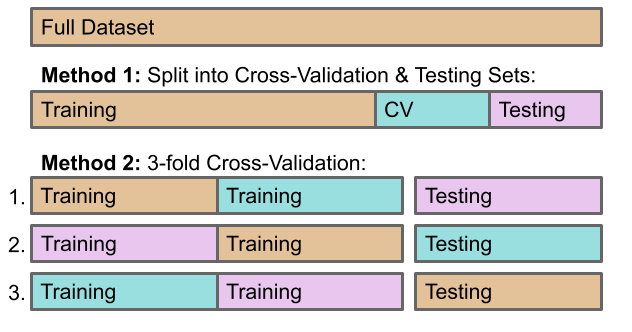
\includegraphics[width=0.85\linewidth]{./chapters/litrev/cverror.png}
  \caption{Illustration of Cross-Validation}
  \label{fig:cverror}
\end{figure}

Using \gls{CV} provides a \textit{\gls{CV} error} that replaces the testing
error during analysis.  As illustrated in Figure \ref{fig:cverror}, this splits
the dataset into $k=3$ subsets. One set is designated as the testing set, and a
model is trained with the rest. Following the first training phase, another
begins, this time with a different subset as the testing set.  In total, this
process in Figure \ref{fig:cverror} is performed $3$ times, giving $3$ models.
The metrics of model performance are averaged by taking the mean of the
accuracy/error of predictions.  This provides an additional level of model
validation than can be achieved with a single testing set. This mean is
reported as the \gls{CV} error. If the \gls{CV} error is acceptable, then
training is performed on the entire training data set and can be tested on new
observations.

\subsubsection{Model Complexity}
\label{sec:complexity}

In statistical learning, there are two sources of error that need to be
simultaneously minimized: bias and variance. Bias is caused by simplifications
in the model, so the error is caused by missed relationships in the data; high
bias is an indication of an underfit model.  Variance is caused by including
random noise in the model, so the error is caused by oversensitivity to that
noise; high variance is an indication of an overfit model. What follows is a
discussion on error considerations that all reduce to one concept: how
\textit{complex should a model be} to best predict a previously unseen test
sample?

\begin{figure}[!htb]
  \makebox[\textwidth][c]{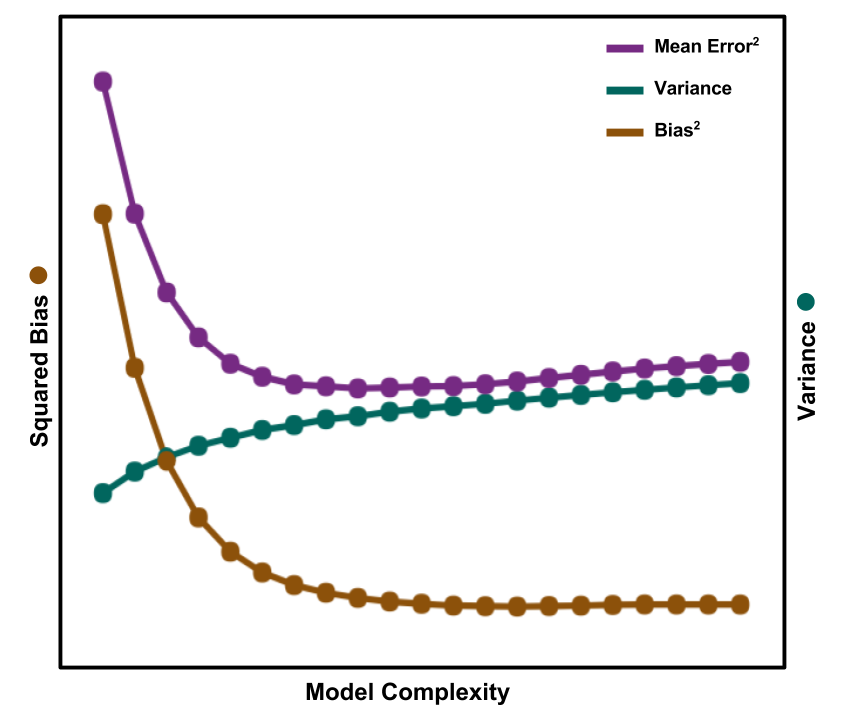
\includegraphics[width=0.7\textwidth]{./chapters/litrev/BVtradeoff.png}}
  \caption{Schematic showing the sources of error, bias and variance, and how 
           they behave with respect to model complexity.}
  \label{fig:bvtradeoff}
\end{figure}

Figure \ref{fig:bvtradeoff} shows the tradeoff between the bias and variance.
The shape of the total error curve has a minimum that we seek to achieve with
our model. Some bias is desired in order to generalize to future unknown data.
But some variance is also positive for the model because it captures the
relationships in the data that the bias counteracts. 

\todo[inline]{transition}
The training set size must be large and diverse enough to be considered
\gls{i.i.d.} because most \gls{ML} algorithms are developed upon this
assumption. Sometimes this is not possible, and the training data are skewed,
i.e., a portion of the data is over-represented. This must be handled
explicitly, but since each algorithm handles skewed data differently, it is
currently beyond the scope of this work. Instead, attempts were made to best
create an \gls{i.i.d.} training set, which is covered in Section
\ref{sec:snflbls}.

\noindent \textbf{Regularization:}
\todo[inline]{Move the text here from wherever you have it stashed}

\noindent \textbf{Diagnostic Plots:} 
\todo[inline]{May or may not include in results, so may or may not include
this. Figures excluded for now.}

Diagnostic plots show the testing errors with respect to some variable on the
\textit{x}-axis.  Typically this variable is related in some way to the model
complexity. This provides insight into the model's fitness, and whether small 
tweaks can be made to increase bias or variance to improve testing performance.
Put another way, these approaches can evaluate under- or over-fitting.

\textit{Learning curves} evaluate the number of training set observations to
include in the training phase. This is relevant in a scenario like this work
where the training set is large (large being a relative term).  The
\textit{x}-axis for learning curves is thus the percentage of the training set
used, or the absolute number of observations included for training. 

\textit{Validation curves} evaluate algorithm hyperparameters that govern model
complexity. This is a good best-practice to implement whether or not the model 
is performing poorly, as a check against overfitting. 

Another area worthy of investigation is the other dimension of the training
set: the number of features included for model training. This is not usually a
value that would be plotted on the \textit{x}-axis of a diagnostic plot (unless
one's data is predisposed to this kind of study), but is considered in this
work. The feature set selection is discussed in Sections \ref{sec:snffeats},
\ref{sec:training2}, and \ref{sec:inforeduc2}.

